%\documentclass[tikz, border=5pt]{standalone}
\usetikzlibrary{angles, quotes, shapes.geometric} % 加载角度、引用、直角标记库
\begin{document}
	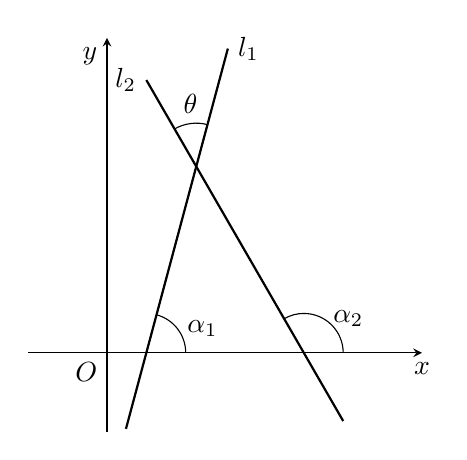
\begin{tikzpicture}[>=stealth, scale=1]
		
		% 1. 绘制坐标轴
		\draw[->] (-1,0) -- (4,0) node[below] {$x$}; % x轴(带箭头和标签)
		\draw[->] (0,-1) -- (0,4) node[below left] {$y$}; % y轴(带箭头和标签)
		\node at (0,0) [below left] {$O$}; % 原点标记
		
		% 2. 绘制直线 \( l_1 \)(倾斜向上)
		\draw[thick] (0.5, 0) --  ++(75: 4) node[right] {$l_1$};
		\draw[thick] (0.5, 0) --  ++(-105: 1) ;
		
		% 3. 绘制直线 \( l_2 \)(倾斜向下,与 \( l_1 \) 垂直)
		\draw[thick] (2.5, 0) -- ++(120: 4) node[ left] {$l_2$};
		\draw[thick] (2.5, 0) -- ++(-60: 1) ;
		
		% 4. 标记角度 \( \alpha_1 \)(\( l_1 \) 与 x 轴正方向的锐角)
		\draw (1, 0) arc (0:75:0.5)  node[midway, right] {$\alpha_1$};
		
		% 5. 标记角度 \( \alpha_2 \)(\( l_2 \) 与 x 轴正方向的钝角)
		\draw (3, 0) arc (0:120:0.5) node[midway, right] {$\alpha_2$}; 
		
		% 6. 绘制夹角标记
		\draw (0.5, 0) --  ++ (75: 3) arc (75:120:0.55) node[midway, above] {$\theta$}; 
		
	\end{tikzpicture}
\end{document}
